対話状態追跡(Dialogue State Tracking ; DST)はユーザの目標と要求を推定するために使用されており,タスク指向対話システムの重要な構成要素である.DSTは各ターンで,ユーザが達成しようとしている目標と,スロットと値のペアとして表される要求を推定することを目指している.通常,この推定は現在のターンでのユーザ発話または前のターンでのシステムの対話行為を考慮して行われる.しかし多くの場合,考慮されたユーザ発話やシステムの対話行為は十分な情報を与えないため,過去の発話を参照する.\par
図\ref{fig:taiwa}の例で示されているように,ユーザはレストランを提案されてからそのレストランに関するさまざまな質問を行う.たとえば今回の対話では,1ターン目のユーザ発話から推定した要求に従って,2ターン目でシステムが “8 Immortals Restaurant” というレストランを提案している.ここからユーザは2ターンに渡ってそのレストランに関する質問を行い,4ターン目で了承する.“restaurant\_name” スロットはユーザが了承したターンでスロット値が更新されるため,現在のターンの発話文だけを考慮すると,値となるレストラン名が見つけられず更新できない.よって,システムは再び2ターン目を参照して “8 Immortals Restaurant” の情報を得る必要がある.通常,このような問題に対処する場合,過去のターンの発話文を対話履歴として入力に加える.しかし,複数ターンの発話文を入力に加えると,スロット値推定に必要な情報を持たない発話 “Unfortunately no” などを入力に含んでしまいノイズとなる.そこで本研究では,過去にスロット値を変更した発話を適切なスロット値推定の手がかりとなる対話履歴として入力に追加するアプローチ\cite{kanren}に影響を受けて,システムの対話行為を用いて重要な対話履歴のみを入力に追加する手法を提案する.\par
また,対話状態追跡のコンペティションである  Dialog System Technology Challenges 8 Track4 Dialogue State Tracking (DSTC8-Track4)\cite{dstc8} が開催されている.本研究では DSTC8-Track4 のタスク設定に基づいて評価を行う.
以下,第 2 章では近年の対話システムにおける対話状態追跡とその問題点について,第 3 章では本研究におけるベースラインとなるモデルについて述べる.また,第 4 章では提案手法について述べる.
第 5 章では対話行為の重要性について調べた予備実験の結果を示し,第 6 章では提案手法の結果と分析を示す.第 7 章では,むすびと今後の課題について述べる.

\begin{figure}[t]
  \centering
  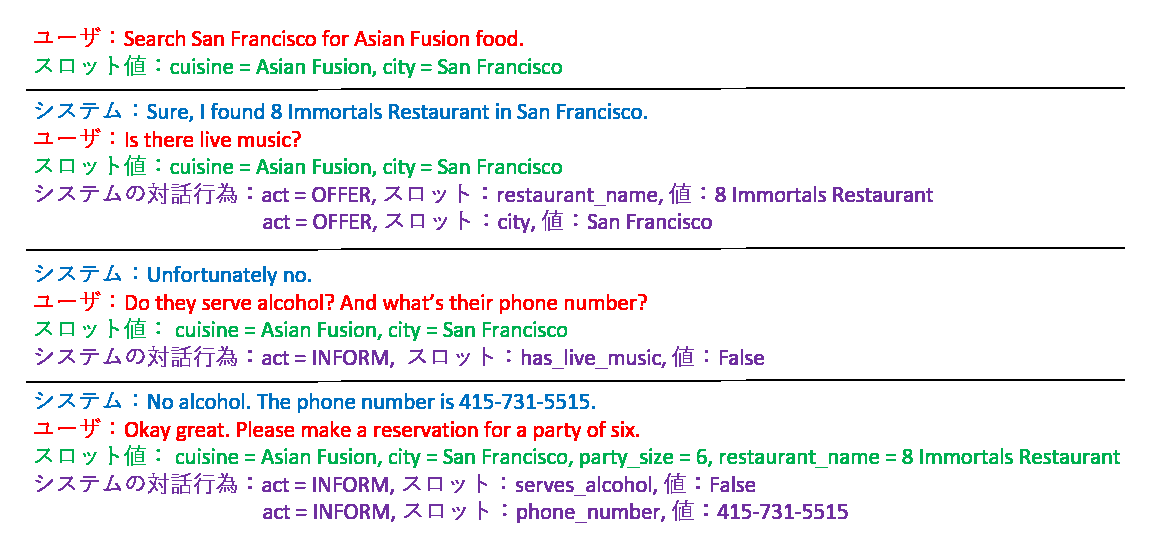
\includegraphics[width=15cm]{chapter1/taiwarei3.eps}
  \caption{SGDデータセットでの対話例.1ターンには,ユーザ発話(赤),システム発話(青),スロット値(緑),システムの対話行為(紫)が含まれる.各ターンは線で分けられている.}
  \label{fig:taiwa}
\end{figure}
